\section{Elliptische Kurven}
\label{sec:para2}
\nextlecture
\subsection{Grundlagen aus der Algebra}
\subsubsection{Polynome}
	Sei $k$ ein beliebiger Körper. \marginnote{[7]}
	
\begin{defn}[Polynom]
	Ein \Index{Polynom} über $k$ in den $n$ Variablen $x_1,\dots,x_n$ ist ein Ausdruck der Form
	\[ f(x_1,\dots,x_n) = \sum\limits_{\nu_1,\dots,\nu_n \geq 0} \alpha_{\nu_1, \dots, \nu_n} x_1^{\nu_1} \cdots x_n^{\nu_n} \]
	mit Koeffizienten $\alpha_{\nu_1,\dots,\nu_n} \in k$, von denen nur endlich viele $\neq 0$ sind. Hat man es mit mehreren Variablen ($n \geq 2$) zu tun, kann man auch kurz
	\[ f(\underline{x}) = \sum_{\uline{\nu} \in \NN_0^n} \alpha_{\uline{\nu}} x_1^{\nu_1} \cdots x_n^{\nu_n} \]
	schreiben, wenn man die Tupelschreibweise $\uline{\nu} \in \NN_0^n$ bzw. $\uline{x} = (x_1, \dots x_n)$ einführt, wobei man für das Monom $x_1^{\nu_1} \cdots x_n^{\nu_n}$ auch kurz $\uline{x}^{\uline{\nu}}$ schreiben kann, wenn klar ist, dass $n \geq 2$ viele Variablen vorliegen. \\
	Die Menge aller Polynome über $k$ in $n$ Variablen wird kurz mit $k[x_1,\dots,x_n]$ oder noch kürzer mit $k[\uline{x}]$ bezeichnet. Wir schreiben dann auch kurz $f \in k[\uline{x}]$, wenn $f(\uline{x})$ ein Polynom ist.
\end{defn}

\begin{bem}
	Durch eine Addition und Multiplikation definiert durch
	\begin{equation}
	\begin{aligned}
		\sum_{\uline{\nu}} \alpha_{\uline{\nu}} \uline{x}^{\uline{\nu}} + \sum_{\uline{\nu}} \beta_{\uline{\nu}} \uline{x}^{\uline{\nu}} &:= \sum_{\uline{\nu}} (\alpha_{\uline{\nu}} + \beta_{\uline{\nu}}) \uline{x}^{\uline{\nu}} \\
		\enbrace*{\sum_{\uline{\nu}} \alpha_{\uline{\nu}} \uline{x}^{\uline{\nu}}} \cdot \enbrace*{\sum_{\uline{\mu}} \beta_{\uline{\mu}} \uline{x}^{\uline{\mu}}} &:= \sum_{\uline{\nu},\uline{\mu}} \alpha_{\uline{\nu}} \beta_{\uline{\mu}} \uline{x}^{\uline{\nu} + \uline{\mu}}
	\end{aligned}
	\end{equation}
	wird $k[\uline{x}]$ zu einem kommutativen Ring mit Eins; das Nullpolynom $0 := \sum_{\uline{\nu}} 0 \uline{x}^{\uline{\nu}}$ ist dabei das Nullelement, das Polynom $1 := 1 \cdot \uline{x}^{\uline{0}} + \sum_{\uline{\nu} \neq 0} 0 \uline{x}^{\uline{\nu}}$ ist das Einselement. \marginnote{"Einspolynom"} \\
	Der Ring $(k[\uline{x}],+,\cdot)$ heißt \Index{Polynomring} über $k$.
\end{bem}

\begin{defn}[Formale Ableitung]
	Für $f(\uline{x}) = \sum_{\uline{\nu}} \alpha_{\uline{\nu}} \uline{x}^{\uline{\nu}} \in k[\uline{x}]$ und $1 \leq j \leq n$ heißt
	\[ \frac{\der f}{\der x_j}(\uline{x}) := \sum_{\uline{\nu}, \nu_j > 0} \alpha_{\uline{\nu}} v_j x_1^{\nu_1} \cdots x_j^{\nu_j-1} \cdots x_n^{\nu_n} \in k[\uline{x}] \]
	die \Index{formale Ableitung} von $f$ nach $x_j$.
\end{defn}

\begin{satz}[Produktregel, Kettenregel]
\label{satz_7.4}
	Für alle $f,g \in k[\uline{x}]$ und $\gamma \in k$ gelten die Ableitungsregeln
	\[ \frac{\der(\gamma f)}{\der x_j} = \gamma \frac{\der f}{\der x_j} \hspace{2cm} \frac{\der(f+g)}{\der x_j} = \frac{\der f}{\der x_j} + \frac{\der g}{\der x_j} \hspace{2cm} \frac{\der(fg)}{\der x_j} = f \frac{\der g}{\der x_j} + g \frac{\der f}{\der x_j} \]
	und für $f \in k[x_1, \dots,x_m], g_1,\dots, g_m \in k[x_1,\dots, x_n]$
	\[ \frac{\der f(g_1,\dots, g_m)}{\der x_j}(\uline{x}) = \frac{\der f}{\der x_1} (g_1,\dots,g_m) \frac{dg_1}{dx_j}(\uline{x}) + \dots + \frac{\der f}{\der x_m} (g_1,\dots,g_m) \frac{\der g_m}{\der x_j}(\uline{x}). \]
\end{satz}

Polynome in einer Variablen $f \in k[x]$ der Form $f(x) = \sum_{\nu = 0}^{k} \alpha_\nu x^\nu$ sind aus den Grundvorlesungen bekannt.
\begin{defn}[Grad]
	Ist $f \neq 0$, so heißt $\deg(f) := \min\{j \in \NN_0 : a_j \neq 0\}$ der Grad von $f$. Für $f \in k[\uline{x}]$ in $n$ Variablen ist $\deg(f) := \min\{\nu_1 + \dots + \nu_n : a_{\uline{\nu}} \neq 0\}$ der \Index{Grad} von $f$. Neu ist bei uns, dass wir uns hier vor allem mit $n = 2$ oder $n = 3$ Variablen beschäftigen werden, wo wir dann auch $f(x,y)$ oder $f(x,y,z)$ schreiben möchten, zum Beispiel $f(x,y) = \alpha_{(2,0)} x^2 + \alpha_{(1,1)} xy + \alpha_{(0,1)}y$. Wir werden dann für die Koeffizienten einfachere Notationen wählen.
\end{defn}

\begin{bem}
	Bleiben wir zunächst beim Polynomring $k[x]$ in einer Variablen $x$. Sei $f \in k[x]$. Wie im Ring $\ZZ$ können wir Teilbarkeit in $k[x]$ studieren und Divisionen mit Rest durchführen (Polynomdivision), daher kann man wie in $\ZZ$ zum Beispiel den ggT von Polynomen mit dem euklidischen Algorithmus ausrechnen. Dies ist aus den Grundvorlesungen bekannt, wir erinnern hier nur an folgendes:
\end{bem}

\begin{defn}[Nullstelle]
	Gegeben sei die Einsetzabbildung
	\begin{equation}
	\begin{aligned}
		k &\longrightarrow k \\
		c &\longmapsto f(c) := \sum_{\nu = 0}^{k} \alpha_\nu c^\nu
	\end{aligned}
	\end{equation}
	Ein Element $c \in k$ heißt \Index{Nullstelle} von $f$, falls $f(c) = 0$ in $k$ ist.
\end{defn}

\begin{bem}
	$c \in k$ ist genau dann Nullstelle, wenn $(x-c)$ ein Teiler von $f$ im Polynomring $k[x]$ ist, d.h. falls ein $g \in k[x]$ existiert mit $(x-c) \cdot g = f$.
\end{bem}

\begin{defn}[Ordnung einer Nullstelle]
	Ist $c$ eine Nullstelle von $f \neq 0$, so gibt es ein maximales $k \geq 1$, sodass $(x-c)^k$ ein Teiler von $f$ ist. Die Zahl $k$ heißt \bet{Ordnung der Nullstelle} $c$. Ist $f(c) \neq 0$, definiert man diese "Nullstellen"ordnung als $0$. \index{Ordnung!Nullstelle}
\end{defn}

\begin{defn}[irreduzibel, prim]
	Ein Polynom $f \in k[x]$ vom Grad $\geq 1$ heißt \Index{irreduzibel} (oder \bet{prim}), falls gilt: Ist $f = u \cdot v$ mit $u,v \in k[x]$, dann ist $\deg(u) = 0$ oder $\deg(v) = 0$, das heißt $f$ kann nicht als Produkt zweier Polynome vom Grad $\geq 1$ geschrieben werden. (vgl. den Begriff "Primzahl" bei $\ZZ$; der Satz von der eindeutigen Zerlegung in irreduzible Polynome heißt der \Index{Satz von Gauß}.)
\end{defn}

Wenn wir $\ZZ$ als Vorbild für den Polynomring $k[x]$ nehmen, möchten wir auch das "Modulorechnen" auf $k[x]$ übertragen, um neue Strukturen zu erhalten. Unsere Moduln sind dann Polynome:
\begin{defn}[Kongruenz, Restklassenring (Polynome)]
	Sei $f \in k[x]$. Dann heißen $a \in k[x]$ und $b \in k[x]$ \bet{kongruent modulo $f$},\index{Kongruenz!Polynome} wenn $f \mid (b-a)$, das heißt falls ein $g \in k[x]$ existiert mit $b = a + fg$.\marginnote{"$\kon$" nur für $\ZZ$} Die Restklassen modulo $f$ sind Teilmengen von $k[x]$ der Gestalt $a + f \cdot k[x] := \{a + fg : g \in k[x]\}$ mit $a \in k[x]$. Das Polynom $a \in k[x]$ heißt ein \Index{Repräsentant} der Restklasse. Ist der Modul $f \in k[x]$ klar, möchten wir dafür auch kurz wieder $\uline{\uline{a}}$ schreiben.\marginnote{doppelt unterstreichen!} \\
	Die Menge der Restklassen modulo $f$ bezeichnen wir mit
	\[ k[x] / (f) := \{a + f\cdot k[x] : a \in k[x]\} = \{\uline{\uline{a}} : a \in k[x]\} \]
	und nennen diese den \bet{Restklassenring modulo $f$}, weil diese bezüglich der Definition $\uline{\uline{a}} + \uline{\uline{b}} := \uline{\uline{a+b}}$ (analog für Multiplikation) für Polynome $a,b \in k[x]$ wieder zu einem kommutativen Ring mit $\uline{\uline{1}}$ als Eins wird. \index{Restklasse!Polynom}
\end{defn}

Doch die einfache Frage, wie viele Elemente der Restklassenring hat, hängt unter anderem vom Körper $k$ ab. Im Fall $k = \FF_p$ beantworten wir diese. Klar ist wegen der Teilbarkeit mit Rest im Ring $k[x]$ (d.h. sind $b,f \in k[x]$ und $f \neq 0$, so existieren eindeutige $g,r \in k[x]$ mit $r = 0$ oder $\deg(r) < \deg(f)$,\marginnote{Polynomdivision} sodass $b = f\cdot g + r$ gilt):
\begin{bem}
\label{bem_7.12}
	Für jede Restklasse $\uline{\uline{a}} = a + f \cdot k[x] \in k[x]/(f)$ gibt es genau einen Vertreter $b \in \uline{\uline{a}} = a + f\cdot k[x]$, das heißt $\uline{\uline{b}} = \uline{\uline{a}}$ bzw. $b + f \cdot k[x] = a + f \cdot k[x]$, mit $b = 0$ oder $\deg(b) < \deg(f)$.
\end{bem}

\subsubsection{Endliche Körper}
\label{subsub:2.1.2}
	Sei nun $k = \FF_p$ mit $p$ prim.

\begin{satz}
	Sei $f \in \FF_p[x]$ irreduzibel mit $r := \deg(f)$. Dann ist $\FF_p[x]/(f)$ ein Körper mit $p^r$ Elementen.
\end{satz}

\minisec{Beweis}
	Dass $\FF_p[x]/(f)$ ein Körper ist, ist klar (Inverse findet man mit dem euklidischen Algorithmus). $\FF_p[x]$ hat $p^r$ Elemente, denn jede Restklasse hat genau einen Vertreter
	\[ b = \underbrace{\alpha_0 + \dots + a_{r-1} x^{r-1}}_{p \text{ Möglichkeiten für jedes } \alpha_j} \qed\]
	
\begin{bem}
	Für jedes $r \in \NN$ gibt es (mindestens) ein irreduzibles Polynom $f \in \FF_p[x]$ mit $\deg(f) = r$.
\end{bem}

\begin{bem}
	Es gibt im Wesentlichen (das heißt bis auf Isomorphie) genau einen endlichen Körper mit $p^r$ Elementen, das heißt welches irreduzible $f$ mit $\deg(f) = r$ wir als Modul nehmen, ist für seine Konstruktion (bis auf Isomorphie!) egal. Wir bezeichnen diesen Körper mit $\FF_{p^r}$.
\end{bem}

\begin{bem}
	Jeder Körper mit endlich vielen Elementen ist einer dieser Körper $\FF_{p^r}$ mit $p$ prim und $r \geq 1$. (ohne Beweis, vgl. Vorlesung "Einführung in die Algebra")
\end{bem}

\begin{bem}
	Wegen Bemerkung \ref{bem_7.12} ist nach Wahl eines irreduziblen Polynom $f \in \FF_p[x], \deg(f) = r$ also
	\[\FF_{p^r} = \{ (\alpha_{r-1} x^{r-1} + \dots + \alpha_1 x + \alpha_0) + f \cdot \FF_p[x] : \alpha_i \in \FF_p\},\]
	die Restklassenvertreter $\alpha_{r-1} x^{r-1} + \dots + \alpha_1 x + \alpha_0$ lassen sich auch durch Koeffizienten-$r$-Tupel $(\alpha_{r-1}, \alpha_{r-2}, \dots, \alpha_1, \alpha_0) \in \FF_{p^r}$ darstellen. Will man mit ihnen stellvertretend für die Polynomrestklassen in $\FF_{p^r}$ rechnen, muss man also erst mit den zugehörigen Polynomen über $\FF_p$ rechnen und modulo $f$ reduzieren.
\end{bem}

\begin{bsp}
	Sei $p = 2, r=3$, wir möchten $\FF_8$ konstruieren.\marginnote{Unterstreichungen weggelassen!} Das Polynom $f(x) = x^3 + x + 1$ ist irreduzibel über $\FF_2 = \{0,1\}$, also ist 
	\[ \FF_8 = \FF_2[x]/(f) = \{ (0,0,0), (0,0,1), (0,1,0), (0,1,1), (1,0,0), (1,0,1), (1,1,0), (1,1,1)\}, \]
	und man rechnet zum Beispiel $(0,1,0) \cdot (1,1,1) = (1,0,1)$, weil
	\[ (0x^2 + 1x + 0) \cdot (x^2 + x + 1) = x^3 + x^2 + x = 1 \cdot (x^3 + x + 1) + (x^2 + 1) \]
	in $\FF_2[x]$ gilt (Division mit Rest durch $f$). \begin{itemize}
	\item Bei Wahl des irreduziblen Polynoms $f(x) = x^3 + x^2 + 1$ ergeben sich zwar andere Rechenregeln für die Vektorenmultiplikation, man erhält aber die selbe "Struktur" bei $+,\cdot$ mit entsprechenden Elementen. Stellen Sie als Übung mal die Multiplikations- und Additionstabellen auf, der Einfachheit halber auch erst mal von $\FF_4$.
	\item Streng genommen müsste man zum Beispiel $\uline{\uline{(\uline{1}, \uline{0}, \uline{1})}} = \uline{\uline{x^2 + \uline{1}}}$ für die Elemente von $\FF_8$ schreiben, um die Reduktion modulo $f$ zu verdeutlichen.
	\end{itemize}
\end{bsp}

\begin{bsp}
	Rechnen in $\FF_{5^3} = \FF_{125}$: Haben wir diesen Körper mit dem irreduziblen Polynom $f = x^3 + x + 1 \in \FF_5[x]$ vom Grad $3$ konstruiert,\marginnote{irreduzibel, da keine Nullstelle und Grad 3!} so rechnen wir in $\FF_{5^3}$ zum Beispiel
	\begin{equation}
	\begin{aligned}
		(1,2,4) \cdot (-1,3,0) &= (x^2 + 2x - 1)(-x^2 + 3x) = -x^4 + 3x^3 - 2x^3 + 6x + x^2 -3x \\
		&= -x^4 + x^3 + x^2 + 3x = (x^3+x+1) \cdot (-x+1) + 2x^2+3x+1 = (2,3,1) \modu f
	\end{aligned}
	\end{equation}
\end{bsp}

\begin{bem}
	Es ist $\Char(\FF_{p^r}) = p$, denn es gilt $\uline{1} + \uline{1} + \dots + \uline{1} = \uline{p \cdot 1} = \uline{0}$, und $p$ ist minimal mit dieser Eigenschaft, da prim.
\end{bem}

\begin{defn}[algebraisch abgeschlossen]
	Ein Körper $k$ ist \Index{algebraisch abgeschlossen}, wenn sich jedes Polynom $f \in k[x], \deg(f) > 0$, als Produkt von linearen Polynomen schreiben lässt, das heißt wenn $f(x) = d(x-c_1) \cdots (x-c_m)$ mit $d,c_i \in k$ gilt.
\end{defn}

\begin{bem}
\label{bem_7.22}
	Man kann jeden Körper $k$ in einen algebraisch abgeschlossenen Körper einbetten. Ein bezüglich "$\subseteq$" minimaler heißt algebraischer Abschluss von $k$, dieser ist eindeutig und wird mit $\overline{k}$ bezeichnet. So ist etwa $\overline{\RR} = \CC$. Der algebraische Abschluss $\overline{\FF_p}$ enthält jeden der Körper $\FF_{p^r}, r \geq 1$, und umgekehrt ist jedes Element von $\overline{\FF_p}$ schon in einem dieser Körper $\FF_{p^r}, r \geq 1$, enthalten. (ohne Beweis)
\end{bem}

\nextlecture
\subsection{Der affine Raum, affine Kurven und der projektive Raum}
	Wir stellen den zweidimensionalen affinen und projektiven Raum vor,\marginnote{[8]} das heißt die wohlbekannte affine Ebene $k^2 = k \times k$ und ihre Ergänzung zur projektiven Ebene $\PP^2(k)$ durch "unendlich ferne Punkte". Kurven im Affinen, wie zum Beispiel elliptische Kurven werden dann in der projektiven Ebene intergriert, weil es rechentechnisch einfacher und mathematisch natürlicher ist.
	
\subsubsection{Der affine und projektive Raum}
	Sei $k$ ein beliebiger Körper. Wir stellen uns meistens $\RR$ vor, weil wir über geometrische Objekte nachdenken möchten; $k$ ist in den Anwendungen aber meist ein endlicher Körper.

\begin{defn}[zweidimensionaler affiner Raum]
	Den zweidimensionalen $k$-Vektorraum $k^2 = k \times k$ schreiben wir auch als $\aff^2(k) := \{(x_1,x_2) : x_1,x_2 \in k\}$ und nennen ihn den \bet{zweidimensionalen affinen Raum} über $k$ bzw. \bet{affine Ebene} über $k$. \index{affiner Raum}
\end{defn}

\begin{defn}[Gerade]
	Eine \Index{Gerade} in $\aff^2(k)$ ist eine Teilmenge der Form
	\[ g(a,b,c) := \{(x,y) \in \aff^2(k) : ax + by + c = 0\} \subseteq \aff^2(k) \]
	für ein Tripel $(a,b,c) \in k^3$ mit $a,b \neq 0$.
\end{defn}

\begin{bem}
	Zwei verschiedene Geraden in $\aff^2(k)$ schneiden sich in genau einem Punkt, es sei denn, sie sind parallel, das heißt dann haben sie keinen gemeinsamen Punkt in $\aff^2(k)$. Soweit nichts Neues.
\end{bem}

\begin{bem}
	Die Ausnahme, dass in der "Ebene" $k \times k$ Geraden parallel sein können, möchten wir uns beim Rechnen gerne ersparen. Wir ergänzen die Ebene um "unendlich ferne Punkte" und erklären, dass sich zwei parallele Geraden in genau so einem Punkt schneiden. Durch diese Ergänzung wird die affine Ebene zur \bet{projektiven Ebene}. Wie kann das sinnvoll so umgesetzt werden, dass alle Punkte Koordinaten bekommen, mit denen man wie üblich rechnen kann, sodass bei der Schnittpunktberechnung auch die unendlich fernen Punkte erhalten werden können?
	\begin{figure}[h]
		\centering
		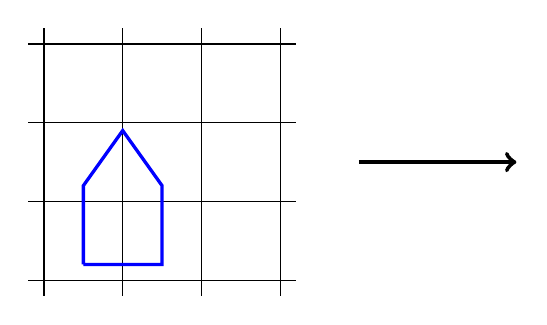
\begin{tikzpicture}
			\foreach \x in {0,1,2,3} {
				\draw (-.2,\x) -- (3.2,\x);
				\draw (\x,-.2) -- (\x,3.2);
			}
			\draw[color=blue,very thick] (.5,.2) -- (1.5,.2) -- (1.5,1.2) -- (1,1.9) -- (.5,1.2) -- (.5,.2);
			
			\draw [ultra thick,->] (4,1.5) -- (6,1.5);
		\end{tikzpicture} \hspace{.3cm}
		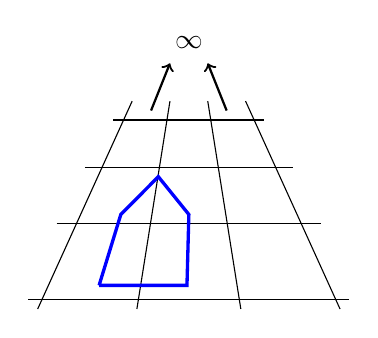
\begin{tikzpicture}[scale=1.2]
			\draw (-.2,0) -- (3.2,0);
			\draw (.1,.8) -- (2.9,.8);
			\draw (.4,1.4) -- (2.6,1.4);
			\draw (.7,1.9) -- (2.3,1.9);
			
			\draw (-.1,-.1) -- (.9,2.1);
			\draw (.95,-.1) -- (1.3,2.1);
			\draw (2.05,-.1) -- (1.7,2.1);
			\draw (3.1,-.1) -- (2.1,2.1);
			
			\draw [color=blue, very thick] (.55,.15) -- (.78,.9) -- (1.177,1.3) -- (1.5,.9) -- (1.48,.15) -- (.55,.15);
			\draw [thick,->] (1.1,2.0) -- (1.3,2.5);
			\draw [thick,->] (1.9,2.0) -- (1.7,2.5);
			\draw (1.5,2.55) node[above]{$\infty$};
		\end{tikzpicture}
		\caption{Ergänzung des zweidimensionalen affinen Raums zur projektiven Ebene.}
	\end{figure}
\end{bem}

Zwei Parallelen $g(a,1,c)$ und $g(a,1,d)$ sollen sich dann schneiden, auch rechnerisch. Wir lösen das so, dass in unserer neuen "Ebene" eine dritte "Koordinate" $z$ hinzukommt, welche bei diesen Parallelen also $=0$ sein müsste, wie folgt:

\begin{defn}[projektive Ebene]
	Die \Index{projektive Ebene} über $k$ ist die Menge
	\[ \PP^2(k) = \{ [y_1 : y_2 : y_3] : y_i \in k \text{ nicht alle } 0\}\]
	mit der Vereinbarung, dass $[y_1 : y_2 : y_3] = [z_1 : z_2 : z_3]$ genau dann gilt, wenn es ein $\lambda \in k \setminus \setnull$ gibt mit $y_1 = \lambda z_1, y_2 = \lambda z_2$ und $y_3 = \lambda z_3$.
\end{defn}

\begin{defn}[projektive Ebene (formal)]
	$\PP^2(k)$ ist die Menge der Äquivalenzklassen in $k^3$ bezüglich der Äquivalenzrelation
	\[ (y_1,y_2,y_3) \sim (z_1,z_2,z_3) \quad :\Leftrightarrow \quad \exists \lambda \in k \setminus \setnull : y_i = \lambda z_i, i = 1, 2, 3 \]
	das heißt $\PP^2(k) := (k^3 \setminus \{(0,0,0)\} / \sim$. \\
	Wir schreiben $[y_1 : y_2 : y_3]$ für die Äquivalenzklasse, die von $(y_1,y_2,y_3)$ repräsentiert wird und nennen sie einen \bet{projektiven Punkt}. $y_1,y_2,y_3$ nennen wir \bet{projektive Koordinaten} von $[y_1: y_2 : y_3]$.
\end{defn}

\begin{bem}
	Ist $y_3 \neq 0$, gilt $[y_1 : y_2 : y_3] = \benbrace*{\frac{y_1}{y_3} : \frac{y_2}{y_3} : 1}$, das heißt die dritte (oder jede andere Koordinate $\neq 0$) kann dann auf $1$ gebracht ("normiert") werden.
\end{bem}

Einem projektiven Punkt $[x:y:z]$ entspricht in unserem Modell in $k^3$ die Ursprungsgerade $\{(\lambda x, \lambda y, \lambda z) : \lambda \in k\}$. Diese Punkte sind entweder $[x:y:1]$ oder $[x:y:0]$ mit $x,y \in k$ (nicht $[0:0:0]$!). \\
Zum Beispiel durch die Abbildung
\begin{equation}
\begin{aligned}
	\iota\colon \aff^2(k) &\longrightarrow \PP^2(k) \\
	(x,y) &\longmapsto [x:y:1]
\end{aligned}
\end{equation}
kann die affine Ebene in die projektive eingebettet werden (d.h. $\iota$ ist injektiv).
\begin{figure}[h]
	\centering
	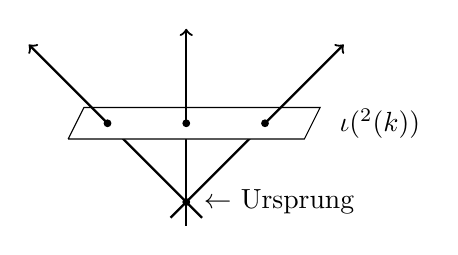
\begin{tikzpicture}
		\draw [thick] (.2,-.2) -- (-1,1);
		\draw [thick] (0,-.3) -- (0,1);
		\draw [thick] (-.2,-.2) -- (1,1);
		
		\draw [fill=white] (-1.5,.8) -- (1.5,.8) -- (1.7,1.2) -- (-1.3,1.2) -- (-1.5,.8);
		
		\draw (-1,1) node[fill,circle,inner sep=1pt]{};
		\draw (0,1) node[fill,circle,inner sep=1pt]{};
		\draw (1,1) node[fill,circle,inner sep=1pt]{};
		\draw (0,0) node[fill,circle,inner sep=1pt]{};
		
		\draw [thick, ->] (-1,1) -- (-2,2);
		\draw [thick, ->] (0,1) -- (0,2.2);
		\draw [thick, ->] (1,1) -- (2,2);
		
		\draw (1.7,1) node[align=left,label={right:$\iota(\aff^2(k))$}] {};
		\draw (.1,0) node[right,align=left] {$\leftarrow$ Ursprung};
	\end{tikzpicture}
\end{figure}

\begin{bem}
	Aber $\PP^2(k)$ enthält zusätzlich noch die projektiven Punkte $[x:y:0]$ mit $x,y \in k$ (nicht $x=y=0$). Offenbar ist $\{[x:y:0] : x,y \in k, \text{ nicht } x = y = 0\}$ eine Gerade in $\PP^2(k)$, die wir \Index{unendlich ferne Gerade} $g_\infty$ nennen möchten, denn mit $j \colon k \rightarrow g_\infty, x \mapsto [x:1:0]$ lässt sich $k$ darin einbetten (das heißt $j$ ist injektiv), wobei auffällt, dass $g_\infty \setminus \im(j)$ aus genau den weiteren Punkt $\oh := [1:0:0]$ besteht, das heißt $g_\infty \setminus \im(j) = \{\oh\}$.
\end{bem}

\begin{bem}
	Somit: $\PP^2(k) = \iota(\aff^2(k)) \sqcup \underbrace{\textcolor{green}{j(k)} \sqcup \textcolor{red}{\{\oh\}}}_{=g_\infty}$ \marginnote{disjunkte Vereinigung}
\begin{figure}[h]
\centering
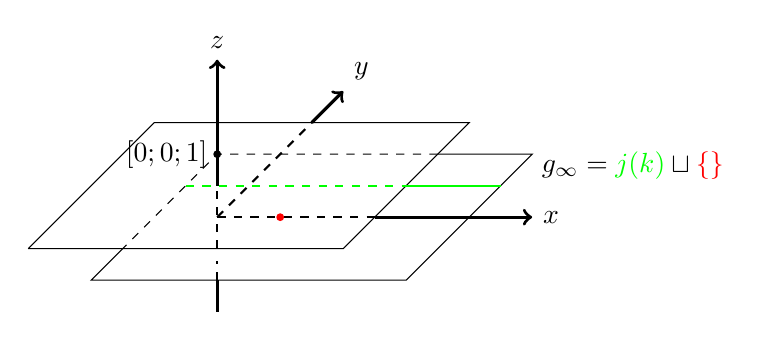
\begin{tikzpicture}[scale=0.8]
	\draw (-1.5,-.5) -- (-2,-1) -- (3,-1) -- (5,1) -- (3.5,1);
	\draw [dashed] (3.5,1) -- (0,1) -- (-1.5,-.5);
	\draw (-3,-.5) -- (2,-.5) -- (4,1.5) -- (-1,1.5) -- (-3,-.5);
	
	
	\draw [very thick] (0,-1.5) -- (0,-1);
	\draw [thick, dashed] (0,-1) -- (0,-.7);
	\draw [thick, dashed] (0,-.5) -- (0,.5);
	\draw [very thick, ->] (0,0.5) -- (0,2.5) node[above] {$z$};
	\draw [thick, dashed] (0,0) -- (2.5,0);
	\draw [very thick, ->] (2.5,0) -- (5,0) node[right] {$x$};
	\draw [thick, dashed] (0,0) -- (1.5,1.5);
	\draw [very thick, ->] (1.5,1.5) -- (2,2) node[anchor=south west] {$y$};
	
	\draw [color=green, thick, dashed] (-.5,.5) -- (3,.5);
	\draw [color=green, thick] (3,.5) -- (4.5,.5);
	
	\draw (1,0) node[fill,circle,inner sep=1pt,color=red]{};
	\draw (1,0) node[color=red,anchor=south west]{$\oh$};
	
	\draw (0,1) node[fill,circle,inner sep=1pt]{};
	\draw (0,1) node [left,align=right] {$[0;0;1]$};
	
	\draw (5,1.2) node[anchor=north west,align=left] {$g_\infty = \textcolor{green}{j(k)} \sqcup \textcolor{red}{\{\oh\}}$};
\end{tikzpicture}
\hspace{1.5cm}
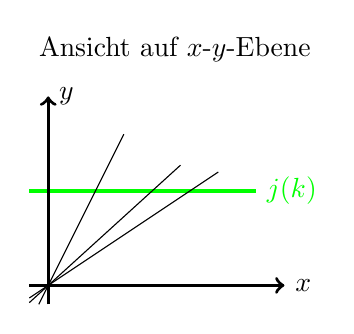
\begin{tikzpicture}[scale=1.2]
	\draw [very thick, color=green] (-.2,1) -- (2.2,1) node[right]{$j(k)$};
	\draw [very thick,->] (-.2,0) -- (2.5,0) node [right] {$x$};
	\draw [very thick,->] (0,-.2) -- (0,2) node [right] {$y$};
	
	\draw (-.1,-.2) -- (.8,1.6);
	\draw (-.2,-.1818) -- (1.4,1.2727);
	\draw (-.2,-.1333) -- (1.8,1.2);
	
	\draw (-.2,2.5) node[right,align=left]{Ansicht auf $x$-$y$-Ebene};
\end{tikzpicture}	
\end{figure}
\end{bem}

Die in $\aff^2(k)$ parallelen Geraden $g(a,1,c) = \{(x,y) \in k^2 : ax + y + c = 0\} = \{(x,-ax-c) : x \in k\}$ und $g(a,1,d)$ müssen die projektiven Punkte $[x:-ax-c:1]$ und $[x:-ax-d:1]$ enthalten. \\
Das klappt, wenn die Gleichung $ax + y \{c,d\} = 0$ zu $ax + y + \{c,d\}z = 0$ ergänzt wird. Sie schneiden sich dann im unendlich fernen Punkt $[1 : -a : 0] = \benbrace*{-\frac{1}{a} : 1 : 0}$, welcher die gemeinsame Steigung $-a$ angibt bzw. die gemeinsame "Richtung" $(1,-a)$. Die gemeinsame Richtung $(1,-a)$ wird zum gemeinsamen Schnittpunkt $\benbrace*{-\frac{1}{a} : 1 : 0}$ erklärt.

\begin{defn}[projektive Gerade]
	Eine \Index{projektive Gerade} ist eine Teilmenge von $\PP^2(k)$ der Form
	\[ g(a,b,c) = \{ [x:y:z] : ax+by+cz = 0\} \text{ für } (a,b,c) \in k^3 \setminus \setnull \]
	Man sagt, die "projektive" Gleichung $ax+by+cz = 0$ ist "durch Homogenisierung" aus $ax+by+c = 0$ entstanden: Durch die Ergänzung mit $z$ haben nun alle Summanden $ax,by,cz$ denselben Grad $1$ als Polynom aus $k[x,y,z]$. Dieses Prinzip werden wir für allgemeinere Kurven für den Übergang vom Affinen ins Projektive übernehmen. Projektive Geraden werden uns in der Form von Tangenten dann wiederbegegnen.
\end{defn}

\minisec{Beispiel und Bemerkung}
	Die projektiven Geraden $g(a,1,c),g(a,1,d)$ schneiden sich in $\penbrace*{-\frac{1}{a}:1:0} \in g_\infty$. Durch je zwei verschiedene Punkte des $\PP^2(k)$ führt genau eine projektive Gerade.
	
\subsubsection{Affine Kurven}
\label{subsub:2.2.2}
	Doch zunächst möchten wir im affinen Raum allgemeinere Kurven untersuchen. Dazu benutzen wir Polynome zu ihrer Beschreibung.
	
\begin{defn}[affine Kurve]
	Sei $f \in k[x,y]$ ein Polynom über $k$ in zwei Variablen $x$ und $y$. Wir bezeichnen die Menge der Nullstellen von $f$ in $k \times k = \aff^2(k)$ als
	\[ \cc_f(k) := \{(u,v) \in \aff^2(k) : f(u,v) = 0\}\]
	Jede solche Nullstellenmenge $\cc_f(k)$ nennen wir eine \Index{affine Kurve}. Ist klar, welches Polynom $f$ vorliegt, schreiben wir auch kurz $\cc(k)$ für $\cc_f(k)$. Geraden sind spezielle affine Kurven (zu linearen Polynomen $f(x,y,z) = ax+by+c$).
\end{defn}

\begin{bem}
	Für uns ist interessant, Kurven über verschiedenen Körpern $k$ zu studieren. Der Fall eines endlichen Körpers ist für Anwendungen interessant, weil dann alle Kurven aus nur endlich vielen Punkten bestehen können.
\end{bem}

\begin{bsp}
	Sei $k = \RR$ und $f(x,y) = y-x^3-x$. Die Nullstellenmenge $\cc_f(k)$ besteht dann aus allen Punkten $(x,y) \in k^2$, welche die Gleichung $y = x^3 + x$ erfüllen. Das reelle Schaubild sieht so aus:
	\begin{figure}[h]
	\centering
	\begin{tikzpicture}[scale=.7]
		\draw [->] (-3,0) -- (3,0) node[above] {$x$};
		\draw [->] (0,-3) -- (0,3) node[right] {$y$};
		\draw [domain=-1.2:1.2,smooth,variable=\x,blue] plot ({\x},{\x*\x*\x + \x});
	\end{tikzpicture}
	\caption{Die Menge $\{(x,y) \in \RR^2 : y = x^3 + x\}$.}
	\end{figure}
	Für $k = \FF_5$ können nur wenige Punkte auf der "Kurve" liegen: Die Tabelle
	\begin{center}
	\begin{tabular}{c|c|c|c|c|c}
	$a$ & $0$ & $1$ & $2$ & $3$ & $4$ \\ 
	\hline $a^3$ & $0$ & $1$ & $3$ & $-3$ & $-1$ \\ 
	\hline $a^3+a$ & $0$ & $2$ & $0$ & 0 & $3$
	\end{tabular} 
	\end{center}
	zeigt, dass $\cc_f(\FF_5) = \{ (0,0), (1,2), (2,0), (3,0), (4,3)\}$ ist, und mit $f_0(x,y) = y^2 - x^3 - x$ haben wir $\cc_{f_0}(\FF_5) = \{(0,0),(2,0),(3,0)\}$. \\
	Ist $\tilde{k} \subseteq k$ ein Teilkörper von $k$ (wie zum Beispiell $\QQ \subseteq \RR$), so folgt auch stets $\cc_f(\tilde{k}) \subseteq \cc_f(k)$. Unsere Kurvenpunkte in $\aff(\FF_5)$ finden wir deswegen zum Beispiel in $\aff(\FF_{25})$ wieder.
\end{bsp}

\begin{defn}[Tangente]
	Eine (affine) \Index{Tangente} an eine affine Kurve $\cc_f(k)$ im Punkt $(a,b) \in \cc_f(k)$ ist die Gerade
	\[ t_f(a,b) = \{ (u,v) : \frac{\der f}{\der x} (a,b)x + \frac{\der f}{\der y}(a,b)y + d = 0\},\]
	falls diese existiert (wir brauchen, dass $\frac{\der f}{\der x}(a,b), \frac{\der f}{\der y}(a,b)$ nicht beide $=0$). Dabei ist $d \in k$ so gewählt, dass $(a,b) \in t_f(a,b)$ gilt.
\end{defn}

\begin{bem}
	Es ist nicht klar, ob Tangenten stets eindeutig existieren. Affine Kurven können sich selbst schneiden oder scharfe "Spitzen" haben. Siehe z.B. Abbildung~\ref{fig:bsp} in Abschnitt~\ref{sec:para0}.
\end{bem}

\begin{defn}[singulärer Punkt]
	Die affine Kurve $\cc_f(k)$ heißt \bet{singulär im Punkt} $(a,b) \in \cc_f(k)$, falls $\frac{\der f}{\der x}(a,b) = \frac{\der f}{\der y}(a,b) = 0$ gilt. \index{singulär}
\end{defn}

\begin{bem}
	Affine Kurven, die in keinem Punkt singulär sind, haben überall eine wohldefinierte Tangente.
\end{bem}

\begin{bem}
	Es kann vorkommen, dass $\cc_f(k)$ gar keine singulären Punkte enthält, wohl aber über einem Erweiterungskörper von $k$, wie etwa $\overline{k}$, dem algebraischen Abschluss über $k$.
\end{bem}

\begin{bsp}
	Für $f(x,y) = y^2 - x^4 - 2x^2 - 1$ hat $\cc_f(\RR)$ keine singulären Punkte: Es ist $\frac{\der f}{\der x}(a,b) = -4a^3 - 4a = -4a(a^2+1), \frac{\der f}{\der y}(a,b) = 2b$. Allerdings sind $(i,0),(-i,0) \in \CC$ singuläre Punkte in $\cc_f(\CC)$, wo $\CC = \overline{\RR}$.
\end{bsp}

\begin{bsp}
	Sei $f(x,y) = y^2 - x^3 - x$ und $k = \FF_p$. Die Ableitungen sind $\frac{\der f}{\der x} (x,y) = -3x^2-1, \frac{\der f}{\der y}(x,y) = 2y$, das heißt die singulären Punkte $(a,b)$ sind die mit $b^2 = a^3 + a$, $-3a^2 = 1, 2b=0$.\begin{itemize}
		\item Für $p \neq 2$ ist $2b = 0$ nur für $b = 0$ richtig, dann ist $0 = a(a^2+1)$ und $3a^2 = -1$. Es folgt $0 = a(3a^2 + 3) = 2a$ und wegen $p \neq 2$ folgt $a = 0$ im Widerspruch zu $3^2=-1$. Also existieren keine singulären Punkte für $p \neq 2$.
		\item Für $p = 2$ ist $\cc_f(\FF_2) = \{(0,0),(1,0)\}$. Es ist $\frac{\der f}{\der x} (1,0) = 0 = \frac{\der f}{\der y}(1,0)$, das heißt $(1,0)$ ist singulärer Punkt.
	\end{itemize}
\end{bsp}

\nextlecture
\subsection{Projektive Kurven}
\subsubsection{Homogene Polynome und projektive Kurven}
\label{sub:2.3} \label{subsub:2.3.1}
	Durch Homogenisierung können wir affine Kurven zu projektiven Kurven machen. \marginnote{[9]}
	
\begin{defn}[homogenes Polynom, Homogenisierung]
	Sei $F \in k[X,Y,Z]$ ein Polynom über $k$ in drei Variablen und $F \neq 0$. Dann heißt $F$ \Index{homogen} vom Grad $d$, falls gilt:
	\[ F(X,Y,Z) = \sum_{v_1,v_2,v_3 \geq 0} \alpha_{v_1,v_2,v_3} X^{v_1} Y^{v_2} Z^{v_3} \]
	und $\alpha_{v_1,v_2,v_3} \neq 0 \Rightarrow v_1 + v_2 + v_3 = d$, das heißt wenn alle Monome in $g$ den Grad $d$ haben.
\end{defn}

\begin{bsp}
	$F(X,Y,Z) = aX + bY + cZ$ ($d=1$) oder $F(X,Y,Z) = Y^2Z-X^3-XZ^2$ ($d=3$).
\end{bsp}

\begin{bem}
	Klar ist, dass ein $f \in k[X,Y]$ durch Ergänzung von $Z$-Potenzen zu einem homogenen Polynom $F_f \in k[X,Y,Z]$ gemacht werden kann: Ist $f(x,y) = \sum_{v_1,v_2 \geq 0} \alpha_{v_1,v_2} x^{v_1} y^{v_2}$ vom Grad $d$, so setze 
	\[ F_f(x,y,z) := \sum_{v_1,v_2 \geq 0} \alpha_{v_1,v_2} x^{v_1} y^{v_2} z^{d-v_1-v_2}.\] Man nennt $F_f$ dann die \Index{Homogenisierung} von $f$. Für diese gilt $F_f(x,y,1) = f(x,y)$.
\end{bem}

\begin{lemma}
	Ist $F \in k[X,Y,Z]$ homogen vom Grad $d$, so gilt für alle $\alpha, \beta, \gamma \in k$ und $\lambda \in k \setminus \setnull$:
	\[ F(\alpha,\beta,\gamma) = 0 \Leftrightarrow F(\lambda \alpha, \lambda \beta, \lambda \gamma) = 0\]
\end{lemma}

\minisec{Beweis}
	Nachrechnen zeigt $F(\lambda \alpha, \lambda \beta, \lambda \gamma) = \lambda^d F(\alpha, \beta, \gamma)$, woraus die Behauptung folgt. \qed

\mbox{}\\	
Somit können wir projektive Kurven definieren:
\begin{defn}[projektive ebene Kurve]
	Sei $F \in k[X,Y,Z]$ homogen. Dann bezeichnen wir die Nullstellenmenge mit
	\[ \cc_F(k) := \{[u:v:w] \in \PP^2(k) : g(u,v,w) = 0\}.\]
	Ist $F$ klar, schreiben wir auch einfach $\cc(k)$ für $\cc_F(k)$. Jede solche Nullstellenmenge heißt eine \Index{projektive ebene Kurve}.
\end{defn}

\begin{bsp}
	Die affine Kurve $\cc_f(x,y)$ zu $f(x,y) = y^2-x^3-x$ kann durch Homogenisieren zu $C_{F_f}(x,y,z)$ mit $F_f(x,y,z) = y^2z-x^3-xz^2$ gemacht werden. Die injektive Abbildung $\iota\colon \aff^2(k) \rightarrow \PP^2(k), (x,y) \mapsto [x:y:1]$ bildet $\cc_f(k)$ nach $\cc_{F_f}(k)$ ab. Die projektive Kurve $\cc_{F_f}(k)$ hat aber noch genau einen weiteren Punkt (auf $g_\infty$), nämlich $[0:1:0]$, das heißt $\cc_{F_f}(k) = \iota(\cc_f(k)) \cup \{[0:1:0]\}$.
\end{bsp}

\begin{lemma}
	$\cc_{F_f}(k) \cap \iota(\aff^2(k)) = \iota(\cc_f(k))$ für jede affine Kurve $\cc_f$ und ihre projektive Kurve $\CC_{F_f}$.
\end{lemma}

\minisec{Beweis}
	$[x:y:1] \in \cc_{F_f}(k) \cap \iota(\aff^2(k)) \Leftrightarrow 0 = F_f(x,y,1) = f(x,y) \Leftrightarrow [x:y:1] \in \iota(\cc_f(k))$. \qed
	
\begin{bem}
	\begin{itemize}
		\item Wir werden hier $\iota$ auch weglassen; es ist klar, was gemeint ist.
		\item Anstelle von $\iota$ können auch die Einbettungen $\iota_2(x,y) = [1:x:y], \iota_3(x,y) = [x:1:y]$ betrachtet werden, das Lemma gilt dann entsprechend.
		\item Geht man für eine projektive Kurve $\cc_F(k)$ zu einer dieser Schnitte mit $\aff^2(k)$ über, so sagt man, man "geht zu affinen Koordinaten" über.
	\end{itemize}
\end{bem}

\begin{defn}[singulärer Punkt, nicht-singulär]
	Sei $F \in k[X,Y,Z]$ homogen vom Grad $d$. Die projektive ebene Kurve $\cc_F(k)$ heißt \bet{singulär im Punkt} \linebreak $P=[a:b:c] \in \cc_F(k)$, falls alle Ableitungen von $F$ in $P$ verschwinden, das heißt
	\[ \frac{\der F}{\der X}(a,b,c) = \frac{\der F}{\der Y}(a,b,c) = \frac{\der F}{\der Z}(a,b,c) = 0.\]
	Die Kurve $\cc_f(k)$ heißt \Index{nicht-singulär}, falls $\cc_F(\overline{k})$ keinen singulären Punkt enthält, wobei $\overline{k}$ einen algebraischen Abschluss von $k$ bezeichnet. \index{singulär}
\end{defn}

\begin{bem}
	Diese Definition hängt nicht davon ab, welche projektive Koordinaten $a,b,c$ eines Punktes $P = [a:b:c]$ betrachtet werden. Sie passt auch mit der alten Definition von "singulären Punkt" für affine Kurven zusammen, wie folgendes Lemma zeigt. Nach dem Lemma genügt es dann, singuläre Punkte, die im Affinen liegen, auf Singularität im Affinen zu testen.
\end{bem}

\begin{lemma}
	Sei $F(X,Y,Z) = \sum_{\uline{v} \geq 0} \alpha_{\uline{v}} X^{v_1} Y^{v_2} Z^{v_3}$ homogen vom Grad $d$ und $f(x,y) = \sum_{\substack{v_1,v_2 \\ v_1 + v_2 \leq d}} \alpha_{v_1,v_2,d-v_1-v_2}x^{v_1} y^{v_2} = F(x,y,1)$, das heißt $F = F_f$. Weiter sei $P \in \cc_F(k)$ mit $P = i(\QQ) \in \iota(\aff^2(k))$. Dann gilt: $\cc_F(k)$ singulär in $P \Leftrightarrow \cc_F(k)$ singulär in $Q$.
\end{lemma}

\minisec{Beweis}
	Haben $Q \in \cc_f(k)$, etwa $Q = (a,b)$, dann ist $P = \iota(Q) = [a:b:1]$. Es ist
	\[ \frac{\der F}{\der X}(X,Y,Z) = \sum_{\substack{v_1 > 0 \\ v_2, v_3 \geq 0}} \alpha_{\uline{v}} v_1 X^{v_1-1} Y^{v_2} Z^{v_3}, \]
	also gilt $\frac{\der F}{\der X}(a,b,1) = \frac{\der f}{\der x}(a,b)$ und entsprechend $\frac{\der F}{\der Y}(a,b,1) = \frac{\der f}{\der y}(a,b)$, sowie
	\[ \frac{\der F}{\der Z}(a,b,1) = \sum_{v_i \geq 0} \alpha_{\uline{v}} v_3 a^{v_1} b^{v_2} = \sum_{v_i \geq 0} \alpha_{v_1,v_2,d-v_1-v_2} (d-v_1-v_2) a^{v_1} b^{v_2} = d \cdot f(a,b) - a\frac{\der f}{\der x}(a,b) - b \frac{\der f}{\der y}(a,b). \]
	Durch Vergleich der Ableitungen folgt die Behauptung in beide Richtungen. \qed
	
\begin{defn}[Tangente]
	Sei $\cc_F(k)$ eine projektive ebene Kurve und $P = [a:b:c]$ ein nicht-singulärer Punkt auf $\cc_F(k)$. Die projektive Gerade $\cc_T(k)$ mit $T(X,Y,Z) := \frac{\der F}{\der X}(a,b,c)X  + \frac{\der F}{\der Y}(a,b,c)Y + \frac{\der F}{\der Z}(a,b,c)Z$ heißt \Index{Tangente} in $P$ an $\cc_F(k)$. Wir schreiben $T_P(\cc_F) := \cc_T(k)$ dafür.
\end{defn}

\begin{bem}
	In nicht-singulären Punkten haben projektive ebene Kurven also eine "schöne" Tangente. Die Voraussetzung "nicht-singulär" braucht man, damit nicht alle drei Ableitungen gleichzeitig verschwinden und so eine projektive Gerade definiert werden kann. Bei Übergang zu affinen Koordinaten erhält man wieder die üblichen (affinen) Tangenten, weil wir dann $Z = 1$ setzen.
\end{bem}

\begin{bsp}
	Sei $\Char(k) \neq 2, f(x,y) := y^2 - 2x^2 - 2, F_f(x,y,z) = y^2-2x^2-2z^2$. Dann ist $(1,2) \in \cc_f(k)$,\linebreak $\frac{\der f}{\der x}(1,2) = -4, \frac{\der f}{\der y}(1,2) = 4$, das heißt $(1,2)$ ist nicht-singulär. Die affine Tangende von $\cc_f$ in $Q = (1,2)$ ist $t_Q(\cc_f) = \{(x,y) \in k^2 : -4x + 4y - 4 = 0\}$, die projektive Tangente von $\cc_F$ in $P = [1:2:1] = \iota(Q)$ ist $T_P(\cc_F) = \{[X:Y:Z] \in \PP^2(k) : -4X + 4Y - 4Z = 0\}$.
\end{bsp}

\begin{mot}
	Wir möchten studieren, wie sich ebene Kurven mit Geraden schneiden und die folgenden Fälle unterscheiden können:
	\begin{figure}[h]
	\centering
	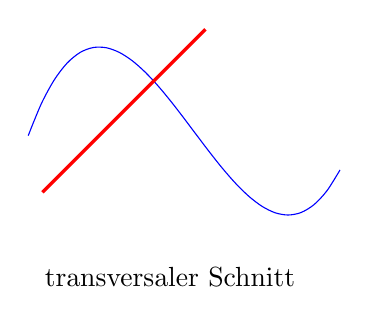
\begin{tikzpicture}[scale=.9]
		\draw[scale=2,domain=-1:1.2,smooth,variable=\x,blue] plot ({\x},{1*\x*\x*\x - .5*\x*\x - 1.25*\x});
		\draw[very thick,domain=-1.8:.5,smooth,variable=\x,red] plot ({\x},{\x+.5});
		\draw (0,-2.5) node[align=center]{transversaler Schnitt};
	\end{tikzpicture}
	\hspace{1cm}
	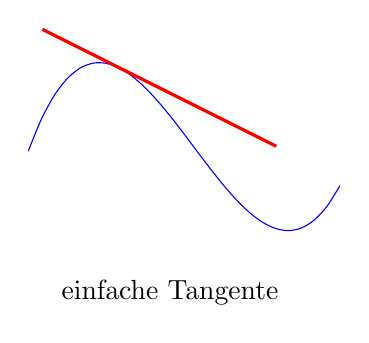
\begin{tikzpicture}[scale=.9]
		\draw[scale=2,domain=-1:1.2,smooth,variable=\x,blue] plot ({\x},{1*\x*\x*\x - .5*\x*\x - 1.25*\x});
		\draw[very thick,domain=-1.8:1.5,smooth,variable=\x,red] plot ({\x},{-0.5*\x + .32});
		\draw (0,-2.5) node[align=center]{einfache Tangente};
	\end{tikzpicture}
	\hspace{1cm}
	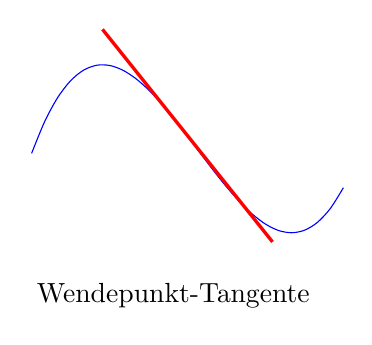
\begin{tikzpicture}[scale=.9]
		\draw[scale=2,domain=-1:1.2,smooth,variable=\x,blue] plot ({\x},{1*\x*\x*\x - .5*\x*\x - 1.25*\x});
		\draw[very thick,domain=-1:1.4,smooth,variable=\x,red] plot ({\x},{-1.25*\x});
		\draw (0,-2.5) node[align=center]{Wendepunkt-Tangente};
	\end{tikzpicture}
	\caption{Wendepunkt-Tangenten liefern gute Approximationen an eine Kurve.}
	\end{figure}
\end{mot}

\begin{defn}[Schnittmultiplizität, Vielfachheit]
	Sei $\cc_F(k)$ eine projektive Kurve zum homogenen Polynom $F \in k[X,Y,Z]$, sei $G(\alpha,\beta,\gamma)$ eine projektive Gerade und $P \in G(\alpha,\beta,\gamma)$ ein Punkt. Ist $P$ kein Schnittpunkt von $\cc_F(k)$ und $G$, setzen wir $m(P;G,\cc_F) := 0$. Ansonsten hat das Polynom $\Psi(t) := F(a+ta', b+tb', c+tc') \in k[t]$ eine Nullstelle in $t = 0$, wobei $P = (a,b,c)$ und $P'=(a',b',c') \in G$ sind. Dann sei $m(P;G,\cc_F)$ die Ordnung der Nullstelle $t = 0$ von $\Psi \in k[t]$, falls $\Psi \neq 0$. Die Zahl $m(P;G,\cc_F)$ heißt \Index{Schnittmultiplizität} bzw. \Index{Vielfachheit}, mit der sich $G$ und $\cc_F$ im Punkt $P$ schneiden.
\end{defn}

\begin{bem}
	Es ist $m(P;G,\cc_F)$ unabhängig von der Wahl von $P'$.
\end{bem}

\begin{bsp}
	Sei $f(x,y) = x(x-1)(x-2)-y \in \RR[x,y]$, das heißt $f(x,y) = x^3 - 3x^2 + 2x - y$ und $F(X,Y,Z) = F_f(X,Y,Z) = X^3-3X^2Z + 2XZ^2-YZ^2$.\\
	Da $\frac{\der f}{\der x} = 3x^2 - 6x + 2, \frac{\der f}{\der y} = -1$, hat $\cc_f$ in $(0,0) \in \cc_f$ die affine Tangente $t_{(0,0)}(\cc_f) = \{(x,y) \in \RR^2 : 2x-y = 0\}$, projektiv aufgefasst lautet die Tangente $T_{(0,0)}(\cc_F) = \{[x:y:z] \in \PP^2(\RR) : 2X-Y + 0Z = 0\} = G(2,-1,0)$. Die Gerade $G(2,-1,0)$ schneidet $\cc_F$ in $[3:6:1]$ und in $[0:0:1]$. Dann haben wir $m([3:6:1];G,\cc_F)=1$, weil
	\begin{equation}
	\begin{aligned}
		\Psi(t) &= F(3+t \cdot 0, 6 + t \cdot 0, 1 + t \cdot 1) \\
		&= 3^3 - 3 \cdot 3^2(1+t) + 2 \cdot 3 \cdot (1+t)^2 - 6 \cdot (1+t)^2 \\
		&= 0 \cdot t^2 + (-3^3 + 6 \cdot 2 - 12)t + (3^3 - 3^3 +6 -6) = -3^3 t^1
	\end{aligned}
	\end{equation}
	eine einfache Nullstelle in $t = 0$ hat, sowie $m([0:0:1];G,\cc_F) = 2$, weil
	\[ \widetilde{\Psi}(t) = F(0+3t,0+6t,1+t) = (3t)^3 - 3(3t)^2(1+t)+2(3t)(1+t)^2-(6t)(1+t)^2 = -3^3 t^2.\]
\end{bsp}

\begin{erl}
	Ist $m(P;G,\cc_F) = 1$, liegt ein transversaler Schnitt der Geraden $G$ mit der Kurve $\cc_f$ vor. Ist $m(P;G,\cc_F) = 2$, so ist $G$ eine "einfache" Tangente an $\cc_F$. Falls $m(P;G,\cc_F) \geq 3$, ist die Tangente eine sehr gute Approximation an $\cc_F$ von "Ordnung $\geq 3$" (da die Schnittmultiplizität genau die Nullstellenordnung von $\Psi(t)$ in $t = 0$ ist).
\end{erl}

\begin{bem}
\label{bem_9.20}
	Ist der Körper $k$ algebraisch abgeschlossen, zerfällt $\Psi$ fast vollständig in Linearfaktoren. Es folgt, dass dann die Summe der Schnittmultiplizitäten aller Schnittpunkte von $G$ mit $\cc_F$ genau $\deg(\Psi) = \deg(F)$ ist, das heißt $\sum_{P \in G \cap \cc_F} m(P;G,\cc_F) = \deg(F)$. Ist $k$ ein beliebiger Körper, so folgt
	\[ \sum_{P \in G \cap \cc_F} m(P;G,\cc_F) \leq \deg(F).\]
\end{bem}

\begin{bem}
	Alle diese Ergebnisse gelten nicht, wenn das lineare Polynom, welches $G$ erklärt, ein Teiler des Polynoms $F$ ist, denn dann lassen sich keine Schnittmultiplizitäten erklären: Ist $G = G(\alpha,\beta,\gamma)$ durch $\alpha X + \beta Y + \gamma Z = 0$ erklärt und $F(X,Y,Z) = (\alpha X + \beta Y + \gamma Z) \cdot H(X,Y,Z)$ für ein $H \in k[X,Y,Z]$, so folgt $G \subseteq \cc_F$ und für $[a:b:c],[a' : b' : c'] \in G$ ist dann
	\[ \Psi(t) = F(a+ta', b+tb',c+tc') = (a(a+ta')+\beta(b+tb') + \gamma(c+tc')) \cdot H(\dots) = 0 \cdot H(\dots) = 0 \]
	das Nullpolynom, also die Nullstellenordnung von $t = 0$ nicht definiert.
\end{bem}

Wir zeigen nun, dass wir bei Tangenten in einem Kurvenpunkt immer die Schnittmultiplizität $\geq 2$ haben, sofern der Grad der Kurve auch $\geq 2$ ist.
\begin{satz}
	Sei $P \in \PP^2(k)$ ein nicht-singulärer Punkt auf $\cc_F$, wobei $\deg(F) \geq 2$ sei, und $T = T_P(\cc_F)$ die Tangente an $\cc_F$ im Punkt $P$. Dann ist $m(P;T,\cc_F) \geq 2$.
\end{satz}

\minisec{Beweis}
	Sei $T = F(\alpha,\beta,\gamma) = \{[X:Y:Z] : \alpha X + \beta Y + \gamma Z = 0\}$ die Tangente in $P = [a:b:c] \in G \cap \cc_F$, also $\alpha = \frac{\der F}{\der X}(a,b,c), \beta = \frac{\der F}{\der Y}(a,b,c), \gamma = \frac{\der F}{\der Z}(a,b,c)$. Sei $Q = [a',b',c'] \in G$ ein beliebiger weiterer Punkt auf $G$, und $\Psi(t) = F(a+ta',b+tb',c+tc')$. Dann ist $\Psi(0) = 0$, da $P \in \cc_F$, und laut Kettenregel (vgl. Satz~\ref{satz_7.4}) ist
	\[ \Psi'(0) = \frac{\der F}{\der X}(a,b,c) \cdot a' + \frac{\der F}{\der Y}(a,b,c) \cdot b' + \frac{\der F}{\der Z}(a,b,c) \cdot c' = \alpha a' + \beta b' + \gamma c' = 0, \]
	weil $Q \in G$. Mit $\Psi(0) = 0, \Psi'(0)=0$ folgt $m(P;T;\cc_F) \geq 2$. \qed

\nextlecture	
\subsubsection{Der Satz von Bézout}
\label{subsub:2.3.2}
	Wir zeigen in diesem Abschnitt, dass Kurven im Allgemeinen nicht allzu viele Schnittpunkte haben: \marginnote{[10]}

\begin{satz}[Satz von Bézout]
\label{satz_10.1}
	Zwei Kurven $\cc_{F_1}, \cc_{F_2}$ in $\PP^2(k)$ können sich in nicht mehr als $\deg(F_1) \cdot \deg(F_2)$ vielen Schnittpunkten treffen, es sei denn, $F_1$ und $F_2$ haben einen gemeinsamen Teiler vom Grad $\geq 1$. Das heißt: \index{Satz von Bézout}
	\[ \ggT(F_1,F_2) = 1 \Rightarrow \#(\cc_{F_1} \cap \cc_{F_2}) \leq \deg(F_1) \cdot \deg(F_2) \]
\end{satz}

\begin{bem}
	Dieser Satz ist eine sehr schwache Form des Satzes von Bézout, welcher besagt: \\
	Sei $k$ ein algebraisch abgeschlossener Körper und seien $F_1,F_2 \in k[X,Y,Z]$ zwei homogene Polynome mit $\ggT(F_1,F_2) = 1$, die zwei ebene projektive Kurven $\cc_{F_1}$ und $\cc_{F_2}$ definieren. Dann ist
	\[ \sum_{P \in \cc_{F_1} \cap \cc_{F_2}} m(P;\cc_{F_1},\cc_{F_2}) = \deg(F_1) \cdot \deg(F_2). \]
	Ist $k$ ein beliebiger Körper, gilt dies mit "$\leq$" statt "$=$".
\end{bem}

\begin{bem}
	\begin{itemize}
		\item Zum Beweis dieses allgemeinen Bézout-Satzes werden mehr Mittel aus der algebraischen Geometrie benötigt, als wir hier zeigen können. Für unsere Zwecke, das Studium elliptischer Kurven, reicht die schwache Version aus Satz~\ref{satz_10.1}, die wir hier beweisen, und insbesondere die spezielle Verschärfung aus Satz~\ref{satz_10.15}.
		\item Die Kurven können singuläre Punkte enthalten.
		\item Den Fall $\deg(F_1) = 1$, das heißt wenn $F_1$ eine Gerade $\cc_{F_1}$ erklärt, haben wir bereits in Bemerkung~\ref{bem_9.20} gezeigt.
		\item Den Begriff der Schnittmultiplizität müsste man für Schnittpunkte zweier beliebiger ebener Kurven verallgemeinern. Wir verzichten hier darauf.
		\item Aus diesem (allgemeinen) Satz von Bézout folgt bereits die schwache Version aus Satz~\ref{satz_10.1}, denn für Schnittpunkte ist $m(P;\cc_{F_1},\cc_{F_2}) \geq 1$, also ist
		\[ \#(\cc_{F_1} \cap \cc_{F_2}) = \sum_{P \in \cc_{F_1} \cap \cc_{F_2}} 1 = \sum_{P \in \cc_{F_1} \cap \cc_{F_2}} m(P;\cc_{F_1},\cc_{F_2}) \leq \deg(F_1) \cdot \deg(F_2).\]
	\end{itemize}
\end{bem}

\begin{bsp}
	Gegeben seien die Parabeln $F_1(X,Y,Z) = X^2 - 3XZ+Z^2-YZ$ und $F_2(X,Y,Z) = -X^2 + 3XZ - 3Z^2 - YZ$ mit den beiden affinen reellen Schnittpunkten $[1:-1:1]$ und $[2:-1:1]$. Laut Bézout-Satz haben die Parabeln noch zwei weitere Schnittpunkte über $\CC$. Diese sind nicht im Affinen, weil die Gleichung $F_1(X,Y,1) = F_2(X,Y,1)$ genau die Lösungen $(1,-1),(2,-1)$ hat. Mit der Gleichung $F_1(X,Y,0) = F_2(X,Y,0) \Leftrightarrow X^2 = -X^2$ erhält man $X = 0$, also den (unendlich fernen) Punkt $[0:1:0] =: \oh$ als einzigen projektiven Schnittpunkt. Eine genaue Analyse würde zeigen, dass $\oh$ die Schnittmultiplizität $2$ hat.
\end{bsp}

\begin{defn}[Resultante]
	Seien $f,g \in k[X]$ Polynome vom Grad $m = \deg(f), n=\deg(g)$, etwa gegeben durch
	\begin{equation}
	\begin{aligned}
		f &= a_mX^m + a_{m-1}X^{m-1} + \dots + a_1X + a_0 \\
		g &= b_nX^n + b_{n-1}X^{n-1} + \dots + b_1X + b_0
	\end{aligned}
	\end{equation}
	Sei
	\[ M(f,g) := \begin{pmatrix}
	a_0 &  &  &  & b_0 &  &  &  \\ 
	a_1 & a_0 &  &  & b_1 & b_0 &  &  \\ 
	\vdots & a_1 & \ddots &  & \vdots & b_1 & \ddots &  \\ 
	a_m & \vdots & \ddots & a_0 & b_n & \vdots & \ddots & b_0 \\ 
	 & a_m &  & a_1 &  & b_n &  & b_1 \\ 
	 &  & \ddots & \vdots &  &  & \ddots & \vdots \\ 
	 &  &  & a_m &  &  &  & b_n
	\end{pmatrix} \in k^{(m+n) \times (m+n)},\]
	das heißt $M(f,g)$ besteht aus $n$ Spalten mit den Koeffizienten von $f$ und $m$ Spalten mit den Koeffizienten von $g$. Dann heißt $\Res(f,g) = \det(M(f,g)) \in k$ die \Index{Resultante} von $f$ und $g$.
\end{defn}

\begin{bem}
\label{bem_10.6}
	\begin{itemize}
		\item Anstelle von $k$ können auch beliebige kommutative Ringe mit $1$ in der Definition stehen.
		\item $\Res(f,g)$ kann als Polynom in den Unbestimmten $a_0,\dots,a_m, b_0, \dots, b_n$ angesehen werden. Für einen darin vorkommenden Term $\prod_{i,j} a_i^{\nu_i} b_j^{\mu_j}$ gilt $\sum_{i=0}^{m} v_i (m-i) + \sum_{j=0}^{n} \mu_j (n-j) = mn$. (ohne Beweis)
	\end{itemize}
\end{bem}

\begin{bsp}
	Sei $k = \RR$, $f(x) = x^2+2x-1$, $g(x) = 4x^3 - 3x + 5$. Dann ist
	\[
		M(f,g) = \begin{pmatrix}
		1 & 0 & 0 & 4 & 0 \\ 
		2 & 1 & 0 & 0 & 4 \\ 
		-1 & 2 & 1 & -3 & 0 \\ 
		0 & -1 & 2 & 5 & -3 \\ 
		0 & 0 & -1 & 0 & 5
		\end{pmatrix} 
	\]
\end{bsp}

\begin{satz}
\label{satz_10.8}
	Sei $S$ ein faktorieller Ring (z.B. Polynomring oder ein Körper), $f,g \in S[X]$ Polynome mit $\deg(f)=m, \deg(g)=n$. Dann sind äquivalent: \begin{enumerate}[(i)]
		\item $f,g, \in S[X]$ haben einen gemeinsamen nichtkonstanten Teiler in $S[X]$
		\item Es gibt $f_0,g_0 \in S[X] \setminus \setnull$ mit $\deg(f_0) \leq m-1, \deg(g_0) \leq n-1$ und $f_0 g= g_0 f$
		\item $\Res(f,g) = 0$
	\end{enumerate}
\end{satz}

\minisec{Beweis}
	\begin{description}
		\item[(i)$\Rightarrow$(ii):] Sei $h$ ein gemeinsamer Teiler, $\deg(h) \geq 1$. Dann setze $f_0 = \frac{f}{h}, g_0 = \frac{g}{h}$.
		\item[(i)$\Leftarrow$(ii):] Sind $f_0,g_0$ wie in (ii) und $h = \ggT(f,g)$, folgt $\ggT\enbrace*{\frac{f}{h},\frac{g}{h}}=1$. Nach Voraussetzung ist $\frac{f}{h} \cdot g_0 = f_0 \cdot \frac{g}{h}$, also ist $\frac{f}{h} \mid f_0$, das heißt $\deg\enbrace*{\frac{f}{h}} \leq \deg(f_0) \leq m-1$, also $\deg(h) \geq 1$.
		\item[(ii)$\Leftrightarrow$(iii):] $f_0, g_0$ entsprechen den nichttrivialen Lösungen des linearen Gleichungssystems
		\[ \sum_{k=1}^{n} c_k T^{k-1} f + \sum_{k=1}^m c_{n+k} T^{k-1} g = 0. \]
		Bezüglich der Basis $T^0, T^1, \dots, T^{n+m-1}$ über $S$ wird das LGS gerade durch $M(f,g)$ beschrieben. \qed
	\end{description}
	
\begin{bew}[von Satz~\ref{satz_10.1}]
	Wir nehmen zum Beweis ohne Einschränkung an, dass $k$ ein unendlicher Körper ist, andernfalls können wir zum Beispiel zum algebraischen Abschluss $\overline{k}$ übergehen, der jedenfalls unendlich ist, vergleiche dazu Bemerkung~\ref{bem_7.22}; denn für eine Körpererweiterung könnte es mehr Schnittpunkte geben. Sei $d_1 = \deg(F_1)$ und $d_2 = \deg(F_2)$. \\
	Angenommen, $\cc_{F_1}$ und $\cc_{F_2}$ hätten mindestens $d_1 d_2+1$ viele Punkte gemeinsam (wir zeigen, dass dann\linebreak $\deg(\ggT(F_1,F_2)) \geq 1$ sein müsste). Seien $P_0, P_1, \dots, P_{d_1d_2}$ Schnittpunkte von $\cc_{F_1}$ und $\cc_{F_2}$.
\end{bew}

\begin{bew}[Fortsetzung]
	Wir können ohne Einschränkung annehmen, dass die Punkte $P_i = (x_i,y_i), i=0,\dots,d_1d_2$, verschiedene\linebreak $x$-Koordinaten und verschiedene $y$-Koordinaten haben (sonst erreicht man dies wieder durch eine Verschiebung bzw. lineare Transformation, da $k$ unendlich ist).
\end{bew}

\begin{bew}[Fortsetzung]
	Wir können eine Gerade $G(\alpha,\beta,\gamma) = \{ [x:y:z] \in \PP^2(k) : \alpha x + \beta y + \gamma z = 0\}$ finden, die durch keine dieser Punkte $P_0, \dots, P_{d_1d_2}$ geht, weil $k$ unendlich ist. Diese Gerade sei ohne Einschränkung $g_\infty$, die unendlich ferne Gerade (durch eine Verschiebung bzw. lineare Transformation lässt sich dies erreichen).
\end{bew}

\begin{bew}[Fortsetzung]
	Somit ist das Problem auf ein affines Problem zurückgeführt worden. Die zugehörigen affinen Kurven seien durch $f_1,f_2 \in k[x,y]$ gegeben, das heißt $f_1(x,y) := F_1(X,Y,1), f_2(x,y) := F_2(X,Y,1)$, mit $\deg(f_1) \leq d_1$,\linebreak $\deg(f_2) \leq d_2$. Wir können ohne Einschränkung sogar $\deg(f_1) = d_1$, $\deg(f_2) = d_2$ annehmen (nach geeigneter Transformation der Koordinaten der Art $X \rightarrow X + \varepsilon Y, Y \rightarrow Y$ ergeben sich für $F_1(X,Y,0) = \sum_{i+j = d_1} c_{ij} X^i Y^j$,\linebreak $F_2(X,Y,0) = \sum_{i+j = d_2} d_{ij} X^i Y^j$ die Terme $(\sum_{i+j = d_1} c_{ij} \varepsilon^i) Y^{d_1}$ in $\widetilde{F_1}(X,Y,0)$ und $(\sum_{i+j=d_2} d_{ij} \varepsilon^i)Y^{d_2}$ in $\widetilde{F_2}(X,Y,0)$).
\end{bew}

\begin{bew}[Fortsetzung]
	Wir betrachten $f_1,f_2 \in (k[x])[y]$ als Polynome in $y$ mit Koeffizienten in $k[x]$ und berechnen die Resultante $R(f_1,f_2) \in k[x]$, diese hat den Grad $d_1 d_2$ in $x$ nach Bemerkung~\ref{bem_10.6}. Sei $R(x) := R(f_1,f_2) \in k[x]$.
\end{bew}

\begin{bew}[Fortsetzung]
	Für jedes $x_i$ haben die Polynome $f_1(x_i,y), f_2(x_i,y) \in k[y]$ eine Faktor $y-y_i \in k[y]$ gemeinsam. Für die $x = x_i$ muss $R(x)$ also verschwinden: $R(x_i) = 0, i=0, \dots, d_1d_2$. Also hat $R(x)$ mehr Nullstellen ($d_1d_2+1$ viele) als sein Grad $d_1d_2$, $R(x)$ muss also das Nullpolynom (in $x$) sein. Aber dann haben $f_1,f_2 \in (k[x])[y]$ einen gemeinsamen Teiler vom Grad $\geq 1$ wegen Satz~\ref{satz_10.8}, (iii) $\Rightarrow$ (i). \qed
\end{bew}

\begin{satz}
\label{satz_10.15}
	Sei $k$ ein beliebiger Körper, $F_1,F_2 \in k[X,Y,Z]$ homogene Polynome mit $d_1 = \deg(F_1), d_2 = \deg(F_2)$ und $\ggT(F_1,F_2) = 1$, und es seien $d_1d_2 - 1$ viele Schnittpunkte von $\cc_{F_1}$ und $\cc_{F_2}$ gegeben. Dann haben sie einen weiteren Schnittpunkt in $\PP^2(k)$ gemeinsam.
\end{satz}

\minisec{Beweis}
	Wir im Beweis von Satz~\ref{satz_10.1} von Bézout erhalten wir ein Polynom $R(x) \in k[x]$ vom Grad $=d_1d_2$. Es hat $d_1d_2-1$ viele Nullstellen $x_1, \dots, x_{d_1 d_2-1}$ laut Voraussetzung, ist also durch $(x-x_1) \cdots (x-x_{d_1d_2-1})$ teilbar, der Quotient ist vom Grad $1$, also $=r \cdot (x-a) \in k[x]$ mit einer (weiteren) Nullstelle $a \in k$.\\
	Somit haben $f_1(a,y), f_2(a,y) \in k[y]$ einen gemeinsamen Faktor vom Grad $\geq 1$. Dieser Grad ist $1$ (denn wäre er $\geq 2$, würde er über $\overline{k}$ in mindestens zwei Linearfaktoren zerfallen, die dann zu zwei weiteren Schnittpunkten mit gleicher $x$-Koordinate $a$ führen würden, sodass es $\geq (d_1d_2-1)+2 > d_1d_2$ viele Schnittpunkte geben müsste -- im Widerspruch zu Satz~\ref{satz_10.1}). Also gibt es nur noch genau einen weiteren Schnittpunkt $(a,y)$ von $\cc_{F_1}$ und $\cc_{F_2}$. \qed